\documentclass[conference]{IEEEtran}

\usepackage{graphicx}
\usepackage{amsmath}
\usepackage{booktabs}
\usepackage{hyperref}
\usepackage{cite}
\usepackage{array}

\title{Correct but Fragile: Numerical Stability Risks in Machine Learning Systems}

\author{
\IEEEauthorblockN{Cordell Stonecipher}
\IEEEauthorblockA{
CSI 4150 -- AI for IT Operations\\
Oakland University\\
Rochester, Michigan, USA
}
}

\begin{document}

\maketitle

\begin{abstract}
Machine learning systems are typically evaluated with aggregate metrics such as accuracy and loss, but those metrics do not guarantee that model behavior is stable under operational variation. This project studies numerical fragility as an MLOps reliability problem and asks whether a model can be operationally inconsistent while remaining superficially correct. A PyTorch-based pipeline was implemented with deterministic training controls, perturbation-based stability scoring, gradient norm tracking, artifact-backed prediction storage, experiment tracking through MLflow, data versioning with DVC, and CI enforcement through GitHub Actions. The final repository artifact set contains completed CPU seed, batch-size, and preprocessing-order sweeps as well as a CUDA precision comparison between \texttt{fp32} and AMP execution. Results show that large prediction disagreement can emerge across seeds, meaningful disagreement can appear across batch sizes and preprocessing order, and a non-zero precision disagreement is also observed under CUDA execution. The current artifact set emphasizes completed CPU-based reproducibility sweeps together with a targeted CUDA precision comparison, so backend-related conclusions are scoped accordingly. The project demonstrates that numerical stability should be treated as a first-class operational signal rather than an afterthought to model quality evaluation.
\end{abstract}

\section{Introduction}

Reproducibility and reliability have become core concerns in modern machine learning practice. As the field has matured, it has become increasingly clear that reporting a strong metric on a benchmark is not enough to ensure that a system behaves consistently when moved across environments, rerun with a different seed, or executed with a different numerical backend. Pineau et al. argue that reproducibility is a prerequisite for reliable scientific progress and for sound experimental claims in machine learning research~\cite{pineau2021}. In operational settings, the same concern becomes a deployment problem: if repeated executions of a training pipeline produce materially different predictions, then downstream systems inherit that instability.

PyTorch's own reproducibility guidance explicitly warns that complete reproducibility is not guaranteed across releases, commits, platforms, or CPU and GPU executions, even under identical seeds~\cite{pytorch_repro}. That warning is often treated as a practical nuisance. In this project, it is treated instead as a systems design problem. The question is not merely how to reduce nondeterminism, but how to observe it, quantify it, and turn it into an enforceable engineering signal.

The project investigates the idea of a model being \emph{correct but fragile}. In other words, a model can appear correct according to accuracy or loss while still exhibiting prediction-level instability under realistic operational changes. To study this, the project builds a stability-aware machine learning pipeline that combines deterministic training controls, perturbation-based numerical sensitivity metrics, cross-run disagreement analysis, experiment tracking, artifact retention, and CI gating.

\section{Problem Statement and Motivation}

The central problem addressed in this work is:

\begin{quote}
How can numerical instability be measured, tracked, and enforced as a reliability constraint in machine learning systems?
\end{quote}

This question matters because production ML systems do not operate in a mathematically ideal environment. They run in toolchains shaped by hardware, software versions, parallelism, floating-point behavior, and configuration drift. If those factors alter predictions in meaningful ways, then a model may not be reliable even if it satisfies benchmark accuracy requirements.

From an AI for IT Operations perspective, this is an operational risk. Silent instability can affect decision support, anomaly detection, triage ranking, or automated actions without triggering an obvious runtime error. The goal of the project is therefore not only to show that instability exists, but also to demonstrate an engineering workflow that exposes it and integrates it into development practice.

\section{System Architecture}

The implemented system combines model execution, artifact generation, experiment tracking, and CI automation in one workflow. The overall architecture is shown in Fig.~\ref{fig:architecture}.

\begin{figure}[t]
\centering
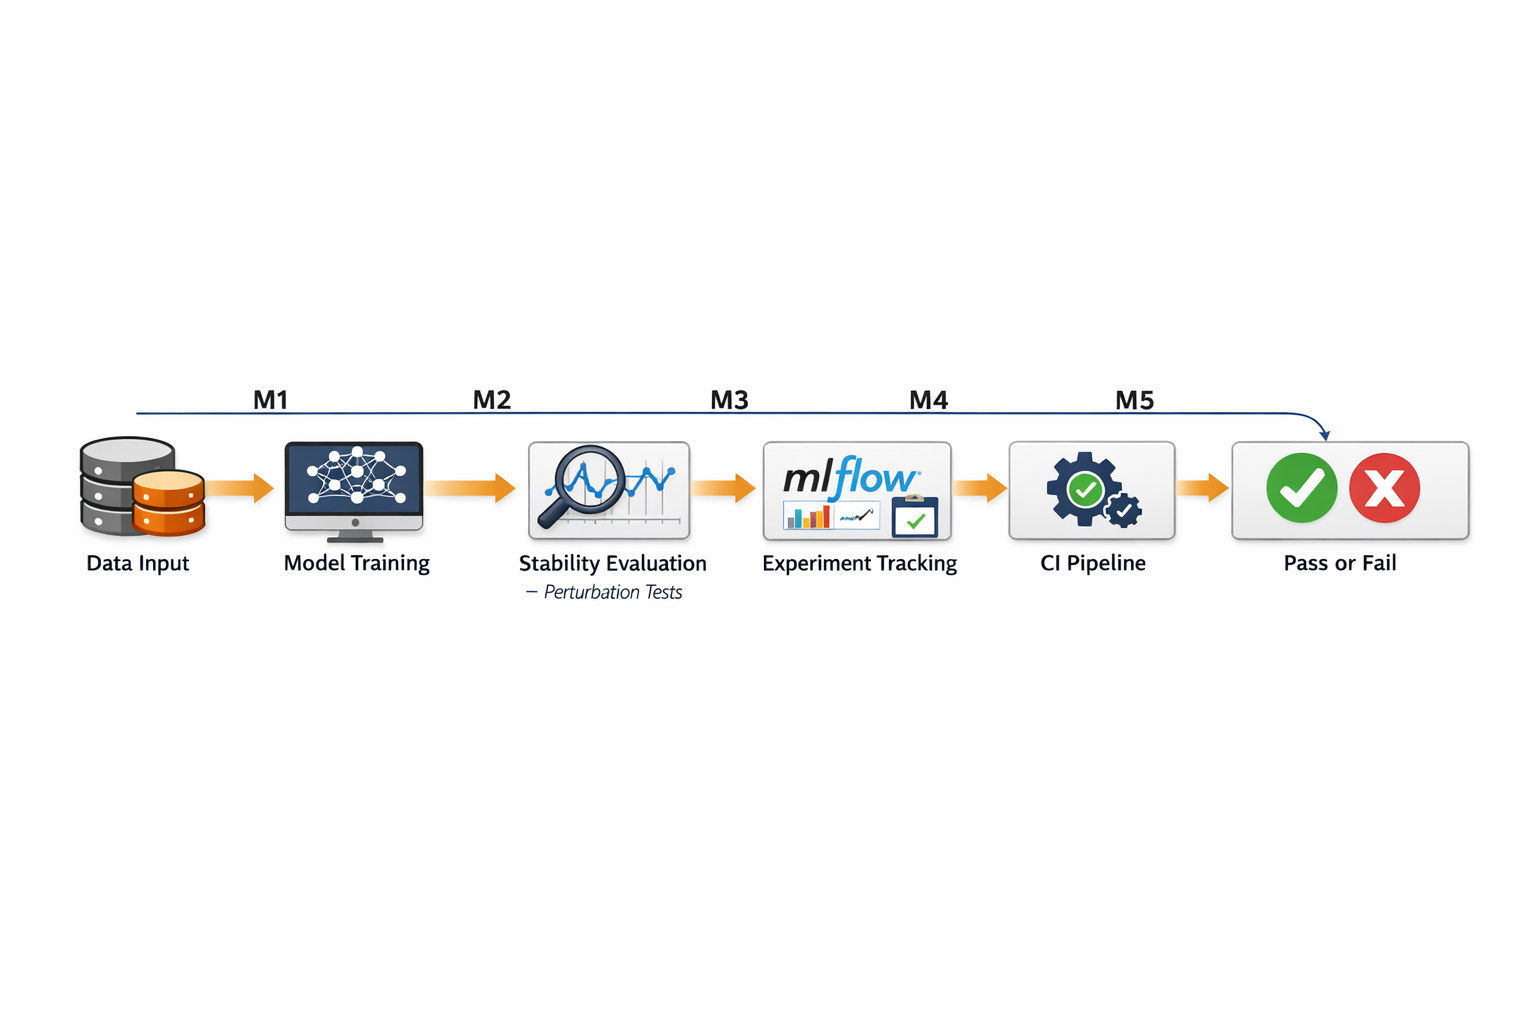
\includegraphics[width=\columnwidth]{images/architecture.png}
\caption{Stability-aware ML pipeline integrating deterministic training, prediction artifact logging, comparison analysis, and CI enforcement.}
\label{fig:architecture}
\end{figure}

The major components are:
\begin{itemize}
\item \textbf{Training and inference:} implemented in PyTorch with explicit seed and determinism controls.
\item \textbf{Artifact logging:} prediction snapshots, logits, and summaries stored per configuration hash.
\item \textbf{Experiment tracking:} MLflow used to log parameters, metrics, and artifacts~\cite{mlflow_tracking}.
\item \textbf{Data versioning:} DVC used to structure data access and reproducible stages~\cite{dvc_start}.
\item \textbf{Automation:} GitHub Actions workflow used to execute validation and enforce perturbation thresholds~\cite{gha_workflows}.
\end{itemize}

This architecture is intentionally operational. Rather than treating stability evaluation as a one-off analysis notebook, the project embeds it into the same tooling stack that would be used for an actual MLOps workflow.

\section{Implementation Details}

\subsection{Model and Dataset}

The core model is a lightweight fully connected network trained on MNIST. A fixed subset of the training data is used so the experimental runtime remains manageable while still allowing systematic sweeps across configuration variables. The objective is not to maximize state-of-the-art accuracy; it is to expose how training behavior changes under controlled operational perturbations.

\subsection{Deterministic Controls}

To reduce avoidable randomness, the training script sets Python, NumPy, and PyTorch seeds and enables deterministic algorithm behavior where possible. cuDNN deterministic settings are also configured. These measures follow the general reproducibility guidance recommended by PyTorch~\cite{pytorch_repro}. The purpose is not to claim perfect determinism across all environments, but to establish a disciplined baseline so that measured drift can be attributed more cleanly to the intended perturbations.

\subsection{Artifact-Backed Design}

Each run stores:
\begin{itemize}
\item predicted labels,
\item logits,
\item a JSON summary containing the configuration and run metrics.
\end{itemize}

Those artifacts are written under a configuration hash and then logged to MLflow. This is a critical design choice. It means that cross-run disagreement can be recomputed later without retraining every model, and it makes the numerical behavior of the system auditable rather than ephemeral.

\subsection{Operational Tooling}

MLflow Tracking provides structured storage for parameters, metrics, and output files, along with a visual comparison interface for runs~\cite{mlflow_tracking}. DVC provides the project with a reproducible pipeline structure around the data and artifact workflow~\cite{dvc_start}. GitHub Actions provides the CI execution model: workflows are defined in YAML, triggered by repository events, and executed as automated jobs~\cite{gha_workflows}.

\begin{figure}[t]
\centering
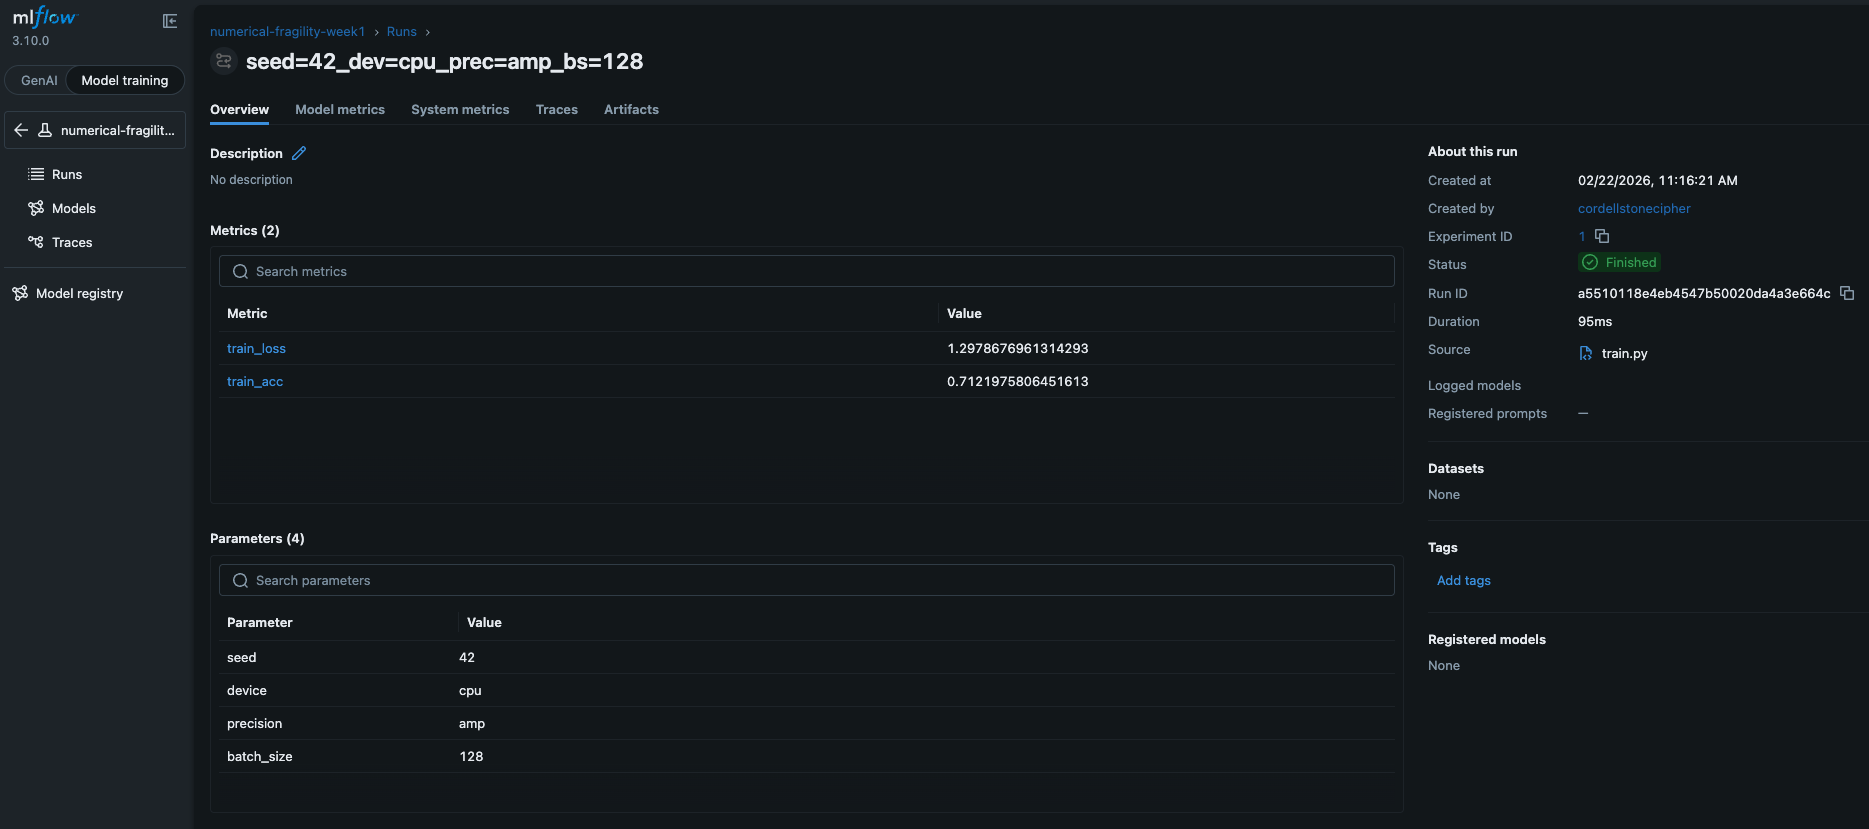
\includegraphics[width=\columnwidth]{screenshots/mlflow_stability_metrics.png}
\caption{MLflow UI used to inspect logged run metrics and stability signals. The screenshot provides a color view of the experiment-tracking layer described in the architecture.}
\label{fig:mlflow}
\end{figure}

Fig.~\ref{fig:mlflow} illustrates the practical value of experiment tracking in this project. The stability metrics are not hidden inside raw logs; they are surfaced alongside standard performance metrics and can be inspected across runs.

\section{Stability Metrics}

The project uses two complementary stability signals.

\subsection{Within-Run Perturbation Sensitivity}

A small perturbation is added to each input:
\begin{equation}
x' = x + \epsilon
\end{equation}

The system then compares the original predictions and perturbed predictions, computing:
\begin{itemize}
\item prediction disagreement rate,
\item mean variance of logits across the two forward passes.
\end{itemize}

This metric captures local numerical sensitivity and is useful for CI enforcement. Even if a run has acceptable accuracy, high perturbation sensitivity suggests fragile behavior near the learned decision boundary.

\subsection{Cross-Run Reproducibility Drift}

Prediction snapshots from completed runs are compared using:
\begin{equation}
\text{Disagreement} =
\frac{1}{N}\sum_{i=1}^{N}\mathbf{1}\left(\hat{y}_{baseline}\neq\hat{y}_{compare}\right)
\end{equation}

This metric measures how much the model's predictions move when operational factors change between runs. In this project, it is applied to seed sweeps, batch-size sweeps, preprocessing-order sweeps, and a CUDA precision comparison.

\section{Experimental Design}

The evaluation matrix is designed around the idea that operational changes should be tested explicitly rather than treated as incidental.

\subsection{Final Artifact Set}

The final repository artifact set is centered on four completed evaluation tracks:
\begin{itemize}
\item a CPU seed sweep,
\item a CPU batch-size sweep,
\item a CPU preprocessing-order sweep,
\item a CUDA precision comparison between \texttt{fp32} and \texttt{amp}.
\end{itemize}

Together, these experiments provide broad coverage of operational fragility across stochastic, configuration, preprocessing, and numerical-precision factors.

\subsection{Why These Sweeps Matter}

Each sweep stresses a different form of fragility:
\begin{itemize}
\item \textbf{Seed sweep:} tests sensitivity to initialization and stochastic training trajectory.
\item \textbf{Batch sweep:} tests sensitivity to optimization dynamics under different mini-batch sizes.
\item \textbf{Preprocessing sweep:} tests whether equivalent-looking preprocessing choices alter prediction behavior.
\item \textbf{Precision sweep:} tests whether numerical representation changes alter prediction behavior.
\end{itemize}

Taken together, these sweeps make the project more than a reproducibility demo. They turn it into an investigation of how operational choices affect prediction consistency.

\subsection{Alignment with the Original Proposal}

The original proposal committed to a broader experimental scope including random seeds, hardware backends, mixed precision, batch sizes, data preprocessing order, prediction variance, disagreement rates, perturbation sensitivity, gradient norm behavior, and reproducibility gaps across repeated configurations. Table~\ref{tab:proposal_alignment} summarizes how those commitments map to the final implementation.

\begin{table}[t]
\centering
\caption{Alignment between proposal commitments and final project scope}
\label{tab:proposal_alignment}
\begin{tabular}{>{\raggedright\arraybackslash}p{0.28\columnwidth}>{\raggedright\arraybackslash}p{0.18\columnwidth}>{\raggedright\arraybackslash}p{0.42\columnwidth}}
\toprule
Proposal Item & Status & Final Treatment \\
\midrule
Seed variation & Completed & Implemented as the main cross-run sweep with stored prediction artifacts. \\
Batch-size variation & Completed & Implemented as the second cross-run sweep with comparison CSV and plots. \\
CPU versus GPU backend analysis & Scoped & Backend-related analysis is represented through CUDA precision artifacts, with conclusions intentionally limited to the collected comparisons. \\
FP32 versus AMP precision analysis & Completed & Implemented through CUDA \texttt{fp32}-versus-AMP comparison within the final artifact set. \\
Data preprocessing order variation & Completed & Implemented as a preprocessing-order sweep with artifact-backed comparison. \\
Prediction variance / disagreement & Completed & Addressed through disagreement rates and stored logits / predictions across runs. \\
Perturbation sensitivity & Completed & Implemented as within-run stability evaluation and used for CI gating. \\
Gradient norm behavior & Completed & Mean and maximum gradient norms are logged per run and summarized in the reporting tables. \\
Reproducibility gaps across identical / controlled configurations & Completed & Addressed through seed, batch, and precision comparisons plus artifact-backed summaries. \\
Git / GitHub / GitHub Actions / Docker / Conda / MLflow / DVC / PyTorch & Completed & Incorporated into the final workflow and documentation, with Git/GitHub providing source traceability and the remaining tools supporting execution, tracking, and reproducibility. \\
\bottomrule
\end{tabular}
\end{table}

This alignment is important for interpreting the final scope correctly. The project delivers the core reliability pipeline proposed at the outset, including reproducibility controls, artifact tracking, CI integration, instability measurement, preprocessing-order experimentation, and gradient norm logging, while keeping backend conclusions appropriately bounded to the artifact set collected.

\section{Results}

\subsection{Aggregate Summary}

Table~\ref{tab:summary} summarizes the final repository disagreement results. The seed sweep dominates the instability profile, while the batch-size and preprocessing-order sweeps produce smaller but still meaningful disagreement. The precision sweep includes only one comparison pair, but even that pair produces a non-zero disagreement rate.

\begin{table}[t]
\centering
\caption{Summary of checked-in cross-run disagreement results}
\label{tab:summary}
\begin{tabular}{lccc}
\toprule
Sweep Type & Comparisons & Mean Drift & Max Drift \\
\midrule
Seed sweep & 4950 & 0.8978 & 0.9124 \\
Batch sweep & 10 & 0.1144 & 0.1698 \\
Preprocessing sweep & 1 & 0.0268 & 0.0268 \\
Precision sweep & 1 & 0.0002 & 0.0002 \\
\bottomrule
\end{tabular}
\end{table}

\subsection{Seed and Batch Drift}

The seed and batch plots in Fig.~\ref{fig:seed} and Fig.~\ref{fig:batch} show the most important empirical result of the project: prediction disagreement can remain large even when the training process appears healthy and overall accuracy stays within a relatively narrow band.

\begin{figure}[t]
\centering
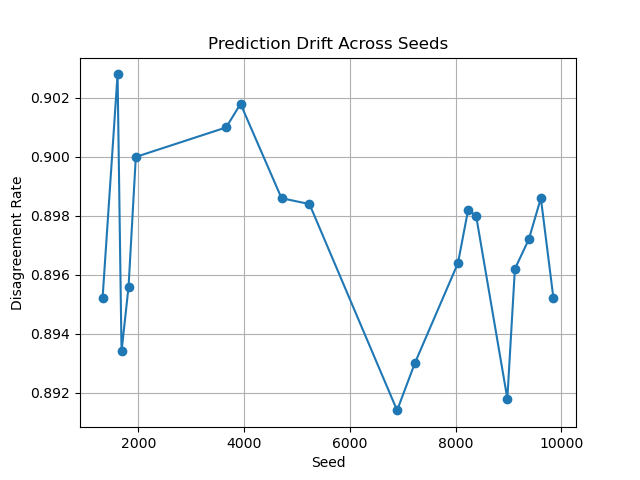
\includegraphics[width=\columnwidth]{images/seed_disagreement.png}
\caption{Prediction disagreement across the seed sweep. The disagreement is extremely high despite broadly similar training accuracy across runs.}
\label{fig:seed}
\end{figure}

\begin{figure}[t]
\centering
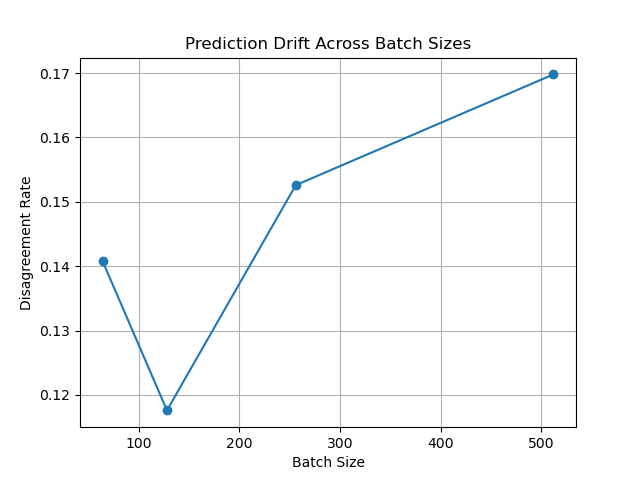
\includegraphics[width=\columnwidth]{images/batch_disagreement.png}
\caption{Prediction disagreement across the batch-size sweep. The disagreement is lower than in the seed sweep but still material.}
\label{fig:batch}
\end{figure}

This distinction matters. A practitioner who looks only at accuracy could conclude that the training pipeline is stable. The disagreement analysis shows otherwise. In effect, two runs can be ``equally good'' in terms of accuracy while disagreeing on a substantial number of individual examples.

\subsection{CUDA Precision Comparison}

Mixed precision is widely used because it can reduce memory use and improve performance on modern accelerators~\cite{micikevicius2018}. The project includes a CUDA precision comparison to determine whether numerical mode changes also alter predictions. As shown in Fig.~\ref{fig:precision}, the disagreement is small in the final repository pair, but it is not zero.

\begin{figure}[t]
\centering
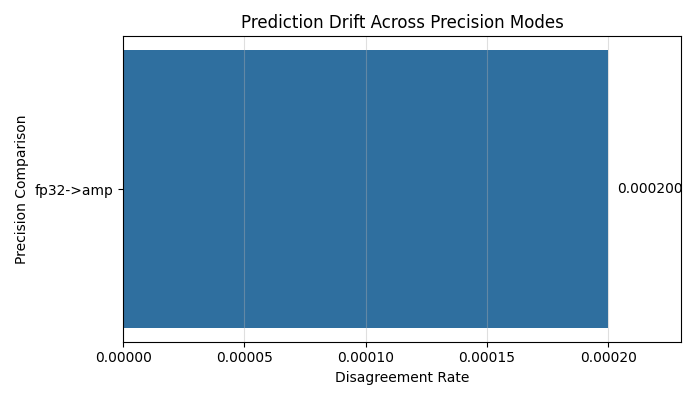
\includegraphics[width=\columnwidth]{images/precision_disagreement.png}
\caption{Prediction disagreement between CUDA \texttt{fp32} and AMP runs. Even with fixed seed and batch size, precision mode changes can affect outputs.}
\label{fig:precision}
\end{figure}

The precision result should be interpreted within the scope of the collected artifact set. It demonstrates that the pipeline can detect prediction differences associated with numerical mode changes and justifies treating precision mode as a first-class experimental variable in reliability evaluation.

\subsection{Preprocessing Order and Gradient Norms}

The project proposal also committed to evaluating preprocessing-order variation and gradient norm behavior. Both are now included in the implementation. A preprocessing-order sweep compares two deterministic normalization sequences and logs the resulting disagreement. In the current artifact set, that sweep produces a disagreement rate of 0.0268, indicating that even modest preprocessing changes can alter predictions.

Gradient norm behavior is also logged for each run through mean and maximum gradient norm metrics. These values are included in the generated summary tables and make optimization dynamics visible alongside stability metrics. The result is not a full optimization-theory study, but it satisfies the proposal's intention of tracking training-time numerical behavior beyond final accuracy.

\subsection{Operational Validation Through CI}

The project does not stop at analysis. Within-run perturbation disagreement is compared against a configurable threshold. If the threshold is exceeded, the run fails. This design turns a numerical signal into an operational gate.

\begin{figure}[t]
\centering
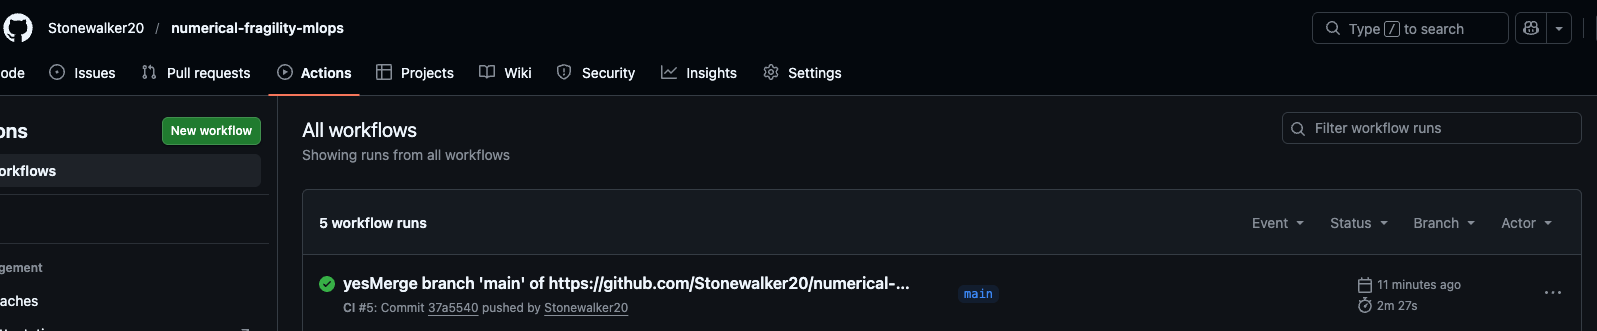
\includegraphics[width=\columnwidth]{screenshots/github_actions_green.png}
\caption{GitHub Actions pipeline used as the automated reliability gate. The workflow validates the project in a clean execution environment.}
\label{fig:gha}
\end{figure}

Fig.~\ref{fig:gha} illustrates the CI dimension of the system. Rather than keeping numerical fragility as a post-hoc diagnostic, the project places it into the same pipeline where engineering teams already enforce quality policy.

\section{Discussion}

Several conclusions emerge from the implementation and results.

First, correctness is not equivalent to stability. The seed sweep in particular shows that a model can remain broadly accurate while becoming highly inconsistent at the prediction level. This supports the core thesis that a model can be correct but fragile.

Second, artifact retention is essential. Without stored predictions and logits, the project would be limited to metric-level analysis. By retaining prediction artifacts, the project can quantify how far runs diverge example by example.

Third, operational tooling adds real value beyond convenience. MLflow makes stability and gradient metrics comparable across runs, DVC structures the artifact workflow, and GitHub Actions converts numerical behavior into a repeatable validation event. These tools are not peripheral to the project; they are part of the argument.

Fourth, precision behavior deserves attention. Although only one CUDA precision pair is available in the final repository set, the result still demonstrates that precision choices can change outputs. That aligns with the broader mixed-precision literature, which emphasizes the numerical tradeoffs that accompany performance gains~\cite{micikevicius2018}.

\section{Limitations}

This study is intentionally scoped as a systems demonstration rather than a large-scale benchmark. The model is lightweight, the dataset subset is constrained to keep sweeps tractable, and the backend evaluation is limited to the comparisons included in the final artifact set. Accordingly, the reported numeric values should be interpreted as evidence of operational fragility within a controlled MLOps setting rather than as universal benchmarks.

However, those limitations do not undermine the main conclusion. Even in a modest setting, the project reveals that operational variation can move predictions in ways that standard aggregate metrics fail to expose. That is the reliability lesson the project is designed to surface.

\section{Future Work}

Several next steps would strengthen the study:
\begin{itemize}
\item extend the study to broader hardware settings,
\item increase the number of precision comparisons,
\item scale to larger models and richer datasets,
\item attach environment metadata to every summary artifact,
\item integrate stability summaries into deployment or registry workflows.
\end{itemize}

\section{Conclusion}

This project demonstrates that numerical instability is a measurable, visible, and enforceable property of machine learning systems. By combining deterministic controls, perturbation-based stability metrics, cross-run disagreement analysis, artifact-backed experimentation, and CI gating, the work provides a practical framework for treating numerical fragility as an MLOps reliability concern. The main conclusion is straightforward: a model can satisfy conventional notions of correctness while remaining operationally fragile, and production-minded ML workflows should measure that fragility explicitly.

\section*{Acknowledgment}

This project was completed individually as part of CSI 4150 -- AI for IT Operations.

\begin{thebibliography}{00}

\bibitem{pineau2021}
J. Pineau, P. Vincent-Lamarre, K. Sinha, V. Larivi\`{e}re, A. Beygelzimer, F. d'Alch\'{e}-Buc, E. Fox, and H. Larochelle, ``Improving Reproducibility in Machine Learning Research,'' \emph{Journal of Machine Learning Research}, vol. 22, no. 164, pp. 1--20, 2021. Available: \url{https://www.jmlr.org/papers/v22/20-303.html}

\bibitem{pytorch_repro}
PyTorch Foundation, ``Reproducibility --- PyTorch Documentation,'' 2025. Available: \url{https://docs.pytorch.org/docs/stable/notes/randomness.html}

\bibitem{mlflow_tracking}
MLflow, ``MLflow Tracking,'' 2025. Available: \url{https://www.mlflow.org/docs/latest/ml/tracking}

\bibitem{dvc_start}
Iterative, ``Get Started with DVC,'' 2025. Available: \url{https://dvc.org/doc/start}

\bibitem{gha_workflows}
GitHub, ``Workflows --- GitHub Actions Documentation,'' 2025. Available: \url{https://docs.github.com/en/actions/concepts/workflows-and-actions/workflows}

\bibitem{micikevicius2018}
P. Micikevicius, S. Narang, J. Alben, G. Diamos, E. Elsen, D. Garcia, B. Ginsburg, M. Houston, O. Kuchaiev, G. Venkatesh, and H. Wu, ``Mixed Precision Training,'' in \emph{International Conference on Learning Representations}, 2018. Available: \url{https://openreview.net/forum?id=r1gs9JgRZ}

\end{thebibliography}

\end{document}
